%------------------------------------------------------------------------------
\chapter{Introduction}
\label{ch:introduction}
\textquote{\textit{A case that can be made for fire being, next to the life process, the most
complex of phenomena to understand}.} - Hoyt Hottle

\begin{figure}[htpb!]
        \centering
        \begin{subfigure}[t]{0.25\textwidth}
                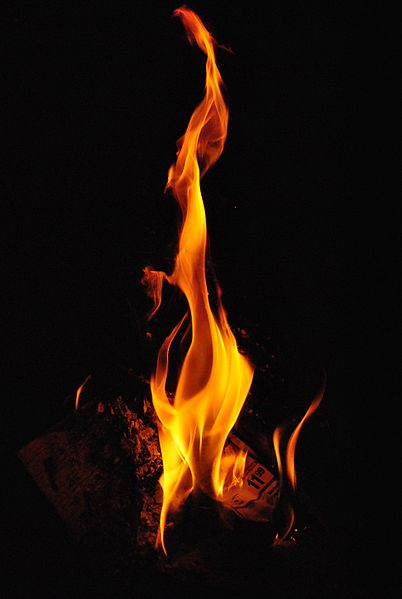
\includegraphics[width=\textwidth]{img/real_fire1}
                \caption{Paper fire~\cite{real_fire1}.}
                \label{fig:real_fire1}
        \end{subfigure}%
        ~ %add desired spacing between images, e. g. ~, \quad, \qquad, \hfill etc.
          %(or a blank line to force the subfigure onto a new line)
        \begin{subfigure}[t]{0.55\textwidth}
                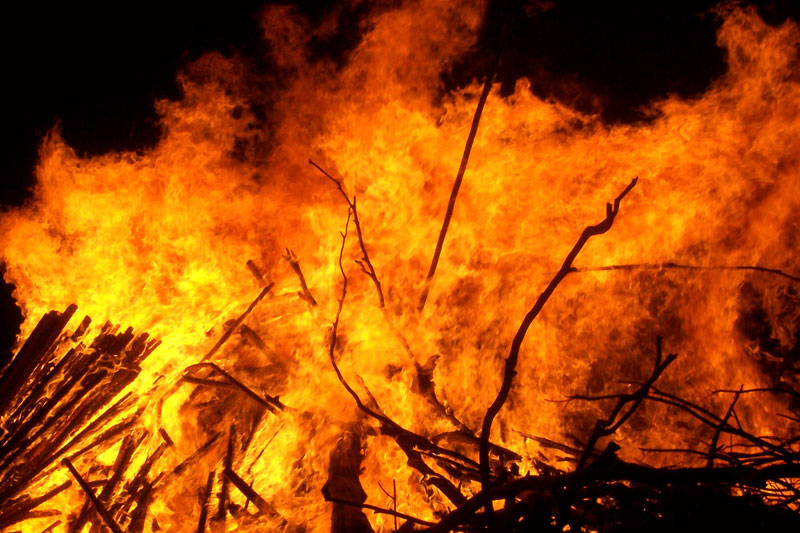
\includegraphics[width=\textwidth]{img/real_fire2}
                \caption{Bone fire~\cite{real_fire2}.}
                \label{fig:real_fire2}
        \end{subfigure}
        \caption{Examples of real fire.}\label{fig:real_fires}
\end{figure}

Computer simulations are widely used to model a diverse range of natural phenomena.
Their popularity lies in their inexpensive nature, predictive capabilities given good mathematical models, parameters can be changed at will to produce new results, the equations governing the system can be modified to create scenarios that are not physically attainable, etc.
Computer generated graphics are used to display the results of the simulations.
Rendering the data on the screen involves transforming a scene into an image that can be displayed using some light transport and illumination model.

For centuries humans has been attracted to fire due to its attractive presence and its dangerous nature, real fire examples are shown in Figure~\ref{fig:real_fires}.
Combustion phenomena are prevalent in daily life, candles, camp fires, explosions, car engines, cooking appliances, etc.
Simulating and visualizing fire related processes has many applications, for example it is widely used for visual effects in the film industry, simulated as part of the virtual environment in the computer games industry; or in the engineering community, where modelling engine combustion and fire safety evaluations are frequently demanded.

Computer generated examples in films include, a planet explosion in Star Trek II, as shown in Figure~\ref{fig:reeves_1983}, where a particle-based technique by~\cite{Reeves:1983} was used; Shrek featured a dragon exhaling fire, as shown in Figure~\ref{fig:lamorlette_2002}, where parametric curves were used to drive the flames~\cite{Lamorlette:2002}; or the more recent work of~\cite{Horvath:2009} based on 2D screen projections for the film Harry Potter and the Deathly Hallows, as shown in Figure\ref{fig:horvarth_2009}.
In these and in many other applications, using real flames is an expensive and hazardous endeavour.

\begin{figure}[htpb!]
        \centering
        \begin{subfigure}[b]{0.3\textwidth}
                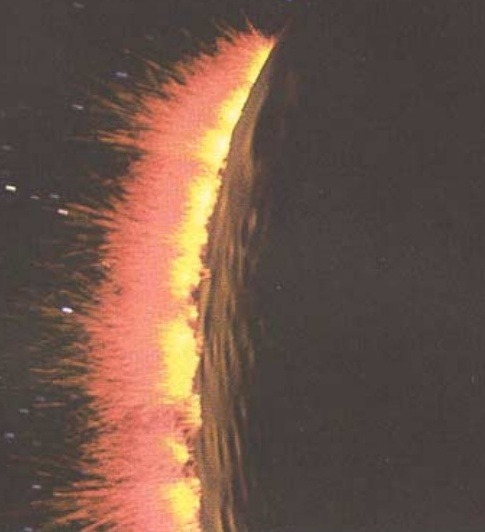
\includegraphics[width=\textwidth]{img/reeves_1983}
                \caption{Explosion in Star Trek II~\cite{Reeves:1983}.}
                \label{fig:reeves_1983}
        \end{subfigure}%
        \quad %add desired spacing between images, e. g. ~, \quad, \qquad, \hfill etc.
          %(or a blank line to force the subfigure onto a new line)
        \begin{subfigure}[b]{0.5\textwidth}
                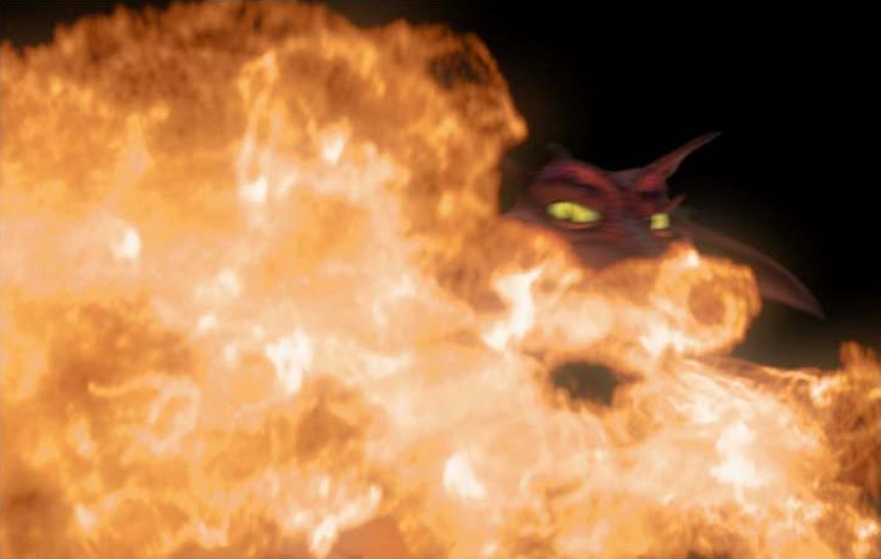
\includegraphics[width=\textwidth]{img/lamorlette_2002}
                \caption{Dragon fire in Shrek~\cite{Lamorlette:2002}.}
                \label{fig:lamorlette_2002}
        \end{subfigure}
        ~ %add desired spacing between images, e. g. ~, \quad, \qquad, \hfill etc.
          %(or a blank line to force the subfigure onto a new line)
        \begin{subfigure}[b]{0.5\textwidth}
                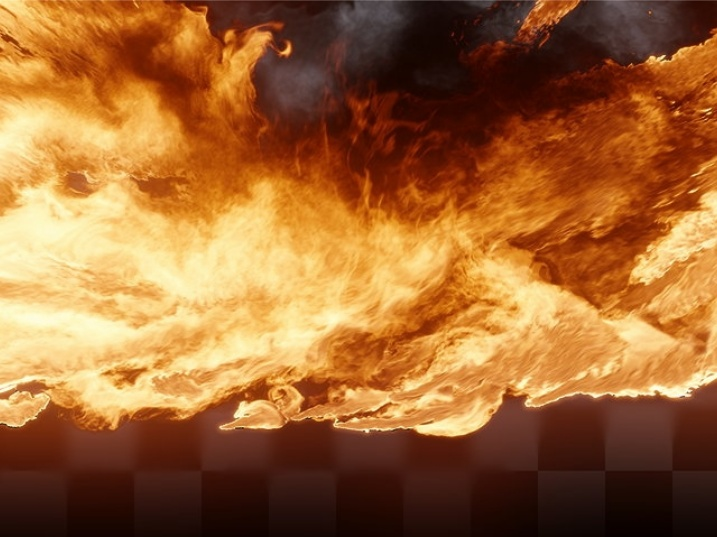
\includegraphics[width=\textwidth]{img/horvarth_2009}
                \caption{Flames in Harry Potter~\cite{Horvath:2009}.}
                \label{fig:horvarth_2009}
        \end{subfigure}
        \caption{Examples of visual effects with fire in the film industry.}
\end{figure}


The computer graphics community have intensively researched the fluid behaviour of water and smoke.
Fire can be also be modelled as a fluid, however due to its multiphase flow, chemical reactions and radiative heat transport, the techniques used for water or smoke cannot be directly applied to flames.
As a result of the aforementioned complexity and the interdisciplinary nature of the problem, fire simulation is still an open problem in computer graphics.

A great deal of work done in the area has sacrificed complexity for interactiveness, therefore producing simplified models which hope to deceit the observer by exploiting the chaotic behaviour present in fire motion.
Nevertheless, physically-based simulations incorporate the intrinsic processes that occur in a combustion scenario:

\begin{description}
\item[Flame motion:]
\item[Fuel erosion:] when the fuel reaches a certain temperature, it is vaporized into a gaseous state, which rises under the influence of buoyancy.
\item[Black body radiation:] the chemical species present in the fuel and the byproducts of the combustions emit energy in various wavelengths.
\end{description}

In order to be able to produce a realistic result, the preceding factors have to be taken into consideration.
In this report a short review in the field of fire simulation and rendering is presented, a state-of-the-art physically-based rendering model by ~\cite{Pegoraro:2006} is discussed in detail, and an implementation of the given model in \Maya is outlined.

TODO Add some fancy pictures from real, film and videogames flames and explosions
TODO Explain everything in more detail and go from slower from general to technical